%\documentclass[AER]{AEA}
\documentclass[11pt]{article}
%\documentclass[12pt]{article}
%\documentclass[12pt,a4paper]{article}

\usepackage{float}
%\usepackage[cmbold]{mathtime}
%\usepackage{mt11p}
\usepackage{placeins}
\usepackage{amsmath}
\usepackage{color}
\usepackage{amssymb}
\usepackage{mathtools}
\usepackage{subfigure}
\usepackage{multirow}
\usepackage{epsfig}
\usepackage{listings}
\usepackage{enumitem}
\usepackage{rotating,tabularx}
%\usepackage[graphicx]{realboxes}
\usepackage{graphicx}
\usepackage{graphics}
\usepackage{epstopdf}
\usepackage{longtable}
\usepackage[pdftex]{hyperref}
%\usepackage{breakurl}
\usepackage{epigraph}
\usepackage{xspace}
\usepackage{amsfonts}
\usepackage{eurosym}
\usepackage{ulem}
\usepackage{footmisc}
\usepackage{comment}
\usepackage{setspace}
\usepackage{geometry}
\usepackage{caption}
\usepackage{pdflscape}
\usepackage{array}
\usepackage[round]{natbib}
\usepackage{booktabs}
\usepackage{dcolumn}
\usepackage{mathrsfs}
%\usepackage[justification=centering]{caption}
%\captionsetup[table]{format=plain,labelformat=simple,labelsep=period,singlelinecheck=true}%

%\bibliographystyle{unsrtnat}
\bibliographystyle{aea}
\usepackage{enumitem}
\usepackage{tikz}
\def\checkmark{\tikz\fill[scale=0.4](0,.35) -- (.25,0) -- (1,.7) -- (.25,.15) -- cycle;}
%\usepackage{tikz}
%\usetikzlibrary{snakes}
%\usetikzlibrary{patterns}

%\draftSpacing{1.5}

\usepackage{xcolor}
\hypersetup{
colorlinks,
linkcolor={blue!50!black},
citecolor={blue!50!black},
urlcolor={blue!50!black}}

%\renewcommand{\familydefault}{\sfdefault}
%\usepackage{helvet}
%\setlength{\parindent}{0.4cm}
%\setlength{\parindent}{2em}
%\setlength{\parskip}{1em}

%\normalem

%\doublespacing
\onehalfspacing
%\singlespacing
%\linespread{1.5}

\newtheorem{theorem}{Theorem}
\newtheorem{corollary}[theorem]{Corollary}
\newtheorem{proposition}{Proposition}
\newcommand{\ra}[1]{\renewcommand{\arraystretch}{#1}}

\newcommand{\E}{\mathrm{E}}
\newcommand{\Var}{\mathrm{Var}}
\newcommand{\Corr}{\mathrm{Corr}}
\newcommand{\Cov}{\mathrm{Cov}}

\newcolumntype{d}[1]{D{.}{.}{#1}} % "decimal" column type
\renewcommand{\ast}{{}^{\textstyle *}} % for raised "asterisks"

\newtheorem{hyp}{Hypothesis}
\newtheorem{subhyp}{Hypothesis}[hyp]
\renewcommand{\thesubhyp}{\thehyp\alph{subhyp}}

\newcommand{\red}[1]{{\color{red} #1}}
\newcommand{\blue}[1]{{\color{blue} #1}}

\newcommand*{\qed}{\hfill\ensuremath{\blacksquare}}%

\newcolumntype{L}[1]{>{\raggedright\let\newline\\arraybackslash\hspace{0pt}}m{#1}}
\newcolumntype{C}[1]{>{\centering\let\newline\\arraybackslash\hspace{0pt}}m{#1}}
\newcolumntype{R}[1]{>{\raggedleft\let\newline\\arraybackslash\hspace{0pt}}m{#1}}

\geometry{left=1.5in,right=1.5in,top=1.5in,bottom=1.5in}
%\geometry{left=1in,right=1in,top=1in,bottom=1in}

\epstopdfsetup{outdir=./}

\newcommand{\elabel}[1]{\label{eq:#1}}
\newcommand{\eref}[1]{Eq.~(\ref{eq:#1})}
\newcommand{\ceref}[2]{(\ref{eq:#1}#2)}
\newcommand{\Eref}[1]{Equation~(\ref{eq:#1})}
\newcommand{\erefs}[2]{Eqs.~(\ref{eq:#1}--\ref{eq:#2})}

\newcommand{\Sref}[1]{Section~\ref{sec:#1}}
\newcommand{\sref}[1]{Sec.~\ref{sec:#1}}

\newcommand{\Pref}[1]{Proposition~\ref{prop:#1}}
\newcommand{\pref}[1]{Prop.~\ref{prop:#1}}
\newcommand{\preflong}[1]{proposition~\ref{prop:#1}}

\newcommand{\clabel}[1]{\label{coro:#1}}
\newcommand{\Cref}[1]{Corollary~\ref{coro:#1}}
\newcommand{\cref}[1]{Cor.~\ref{coro:#1}}
\newcommand{\creflong}[1]{corollary~\ref{coro:#1}}

\newcommand{\etal}{{\it et~al.}\xspace}
\newcommand{\ie}{{\it i.e.}\ }
\newcommand{\eg}{{\it e.g.}\ }
\newcommand{\etc}{{\it etc.}\ }
\newcommand{\cf}{{\it c.f.}\ }
\newcommand{\ave}[1]{\left\langle#1 \right\rangle}
\newcommand{\person}[1]{{\it \sc #1}}

\newcommand{\AAA}[1]{\red{{\it AA: #1 AA}}}
\newcommand{\YB}[1]{\blue{{\it YB: #1 YB}}}

\newcommand{\flabel}[1]{\label{fig:#1}}
\newcommand{\fref}[1]{Fig.~\ref{fig:#1}}
\newcommand{\Fref}[1]{Figure~\ref{fig:#1}}

\newcommand{\tlabel}[1]{\label{tab:#1}}
\newcommand{\tref}[1]{Tab.~\ref{tab:#1}}
\newcommand{\Tref}[1]{Table~\ref{tab:#1}}

\newcommand{\be}{\begin{equation}}
\newcommand{\ee}{\end{equation}}
\newcommand{\bea}{\begin{eqnarray}}
\newcommand{\eea}{\end{eqnarray}}

\newcommand{\bi}{\begin{itemize}}
\newcommand{\ei}{\end{itemize}}

\newcommand{\Dt}{\Delta t}
\newcommand{\Dx}{\Delta x}
\newcommand{\Epsilon}{\mathcal{E}}
\newcommand{\etau}{\tau^\text{eqm}}
\newcommand{\wtau}{\widetilde{\tau}}
\newcommand{\xN}{\ave{x}_N}
\newcommand{\Sdata}{S^{\text{data}}}
\newcommand{\Smodel}{S^{\text{model}}}

\setlength{\parindent}{0.0cm}
\setlength{\parskip}{0.6em}

\numberwithin{equation}{section}
\DeclareMathOperator\erf{erf}
%\let\endtitlepage\relax

\begin{document}

%\onehalfspacing
\begin{titlepage}
\title{Preference Reversal and Temporal Discounting by Optimizing Growth Rates}
\author{Alexander Adamou \and Yonatan Berman \and Diomides Mavroyiannis \and Ole Peters}
%\date{First version: August 26, 2018\,\,\,\,\,\,\,\,\,\,\,\,\,\,\,\,\,\,\,\,\,\,\,\,Last revised: \today}
%\date{\today\\\href{https://www.dropbox.com/s/epq42goae2px35i/mobility_recov.pdf?dl=0}{Click here for most recent version.}}
%\date{}
\date{\today}
\maketitle
\begin{abstract}
\noindent An important question in economics is how people evaluate payments in the future. The standard phrasing of the problem is in part psychological: the value we attach to a future payment is the dollar value of the payment discounted by a factor whose functional form is determined by our subjective psychology and whose (objective) argument is how long we have to wait for the payment. The functional form is called the ``discounting function'', in practice commonly exponential or hyperbolic. Here we present an interpretation of these forms in terms of growth rates. A payment in the future, we posit, is often viewed as a growth rate of wealth averaged over the time until the payment. Choosing the greatest multiplicative growth rate is mathematically equivalent to exponential discounting, and the additive growth rate is equivalent to hyperbolic discounting. Multiplicative and additive processes are important models for wealth, corresponding approximately to non-earned and earned income. More complicated growth processes result in different discounting functions.
\\
\\
\noindent\textbf{Keywords: Decision theory, Hyperbolic discounting, Ergodicity economics}
\\
%\noindent\textbf{JEL Codes:} D3, E2, H0, J6\\

\bigskip
\end{abstract}
\setcounter{page}{0}
\thispagestyle{empty}
%\nopagebreak
\end{titlepage}
\pagebreak \newpage
%\nopagebreak

\section{Introduction}\label{sec:introduction}

Preference reversal (\textit{PR}) is a behavioral phenomenon documented during the past half a century in many studies in economics and psychology~\citep{lichtenstein1971reversals,lindman1971inconsistent,grether1979economic,loomes1983rationale,tversky1990causes,ainslie1992picoeconomics,laibson1997golden}. It takes various forms in different contexts. In its original psychological context~\citep{tversky1969intransitivity,lichtenstein1971reversals} it refers to the intransitivity in decision making under uncertainty. It also refers to the phenomenon in which a decision maker changes mind between two options in time.

Observed PR phenomena puzzled economics, leading to various explanations and theories. One theory that gives rise to PR is hyperbolic discounting~\citep{ainslie1992picoeconomics,sozou1998hyperbolic,laibson1997golden}, suggesting that the valuation of choices falls hyperbolically in time. This means that decision makers may favor earlier guaranteed reward over higher later reward, in a way that is inconsistent with standard economic theory. Hyperbolic discounting has been established as a plausible explanation for PR. 
Yet, the dynamically inconsistent preferences it induces had challenged standard economic theory~\citep{laibson1997golden,starmer2000developments,thaler2016behavioral}. This questions some of the basic axioms of expected utility theory, which predicts exponential discounting, \ie valuation of choices that falls exponentially in time.
%In what sense does EUT predict exponential discounting?

\citet{rubinstein2003economics} suggested that the same experiments used as evidence for supporting the validity of hyperbolic discounting, can also be used to reject it under different axioms. In addition, various behavioral explanations for hyperbolic discounting have been given in the economic literature. One approach is to place the conditions on the information of decision makers.~\citet{sozou1998hyperbolic,dasgupta2005uncertainty} suggested that a decision maker is learning over time, which allows for PR. This approach implicitly assumes constructivist rationality similar to that of~\citet{smith2003constructivist}. In the most basic sense, the methodological approach is to posit the cognitive situation of the agent and to deduce his discounting rule.

The reasoning behind the model of~\citet{sozou1998hyperbolic}, for example, is that agents do not know the hazard rate of an event and learn about the hazard rate over time. The logic behind this is that the agents use Bayesian updating to gradually learn over time, the longer an event does not occur, the more likely it is that it will not occur (decreasing hazard rate). Using this approach, it is shown that an exponential distribution yields hyperbolic discounting.

On the other hand,~\citet{dasgupta2005uncertainty} assume that the agent knows that an event will occur for certain but it is unclear when. The mechanics behind the model are that since an event will occur at some future time, the closer we are to that future time the more certain one of the events will occur very soon. This is because it is initially assumed that the probability of early realizations is the same for both gambles. This, in turn, means that the chance for early realization is more valuable for larger payouts than smaller payouts. They later extend their result to say that the density is not the same but that the probability of one event increases relatively more over time which allows for a wider class of hazard functions. This provides a model for how hyperbolic discounting can describe PR under uncertainty.

This paper takes a different approach. Our model consists of a decision maker, who chooses between two known and different payoffs to be received at known and different times by comparing the growth rates of total wealth associated with each option. The model is further specified by assumptions about the wealth dynamics of the decision maker and the time frame of the decision. In some specifications, the model produces forms of discounting -- including hyperbolic -- which predict PR. In another specification, standard exponential discounting under multiplicative growth is recovered, which does not predict PR. Thus, we propose that a model that assumes a growth rate maximizing decision maker under various assumptions is consistent with a wide range of experimental evidence.

This approach is similar to~\citet{Radner1998} -- he assumed that firms maximize their survival rate, which is a special case of maximizing the growth rate. To see why we note that if a strategy results in non-survival, then the growth rate for it will be zero. 
XXX OP: zero growth rate means maintaining status quo, not death... XXX
He further shows that firms that maximize the probability of survival, will outcompete those which maximize profits and hence, in the long run there will only be survival maximizing firms.
XXX OP: not sure this is true, but I don't know what the terms mean. I can easily imagine a situation where I can guarantee survival at zero growth, and a little risk gets a big reward, which may well lead to outperformance despite the risk of non-survival.XXX

The main contribution of this paper is to shed new light on the possible explanations for PR and hyperbolic discounting, while demonstrating this can be achieved without being inconsistent with the standard exponential discounting. The importance of these findings lies in the absence of rationality criteria -- the same model and the same criteria can produce different types of discounting. We stress that the importance lies in specifying the dynamics of the problem in question.

The paper also contributes to the growing branch of ergodicity economics~\citep{peters2016evaluating,berman2016far,peters2018time}, which proposes an alternative to mainstream decision theories, such as expected utility theory and prospect theory, namely that agents maximize the growth of their resources averaged over time. This joins recent evidence on the effect changes in the dynamics of wealth have on decision makers under uncertainty~\citep{hulme2019unpublished}.

The paper is organized as follows.~\Sref{model} lays out our model and the basic setup of the problem we are addressing. In~\Sref{results} we present different specifications for the problem in question. We describe how a decision maker will discount payoffs in each specification under our model, giving rise to preference reversal. We conclude in~\Sref{discussion}.

\section{Model}\label{sec:model}

Our model consists of a decision maker facing a choice between two options, labelled $a$ and $b$, at time $t_0$. Option $a$ guarantees a fixed and known payout of $\Dx_a$ after time period $\Dt_a$. Option $b$ guarantees a fixed and known payout of $\Dx_b$ after time period $\Dt_b$. We assume that a larger and earlier payout is always preferred, so we confine our attention to cases where $\Dx_b > \Dx_a$ and $\Dt_b > \Dt_a$. We also assume that the decision maker knows his total net wealth at time $t_0$, which we denote by $x\left(t_0\right)$. In general, $x\left(t\right)$ denotes the wealth of the decision maker at time $t$. This setup is illustrated in~\fref{basicsetup}.

\begin{figure}[!htb]
\centering
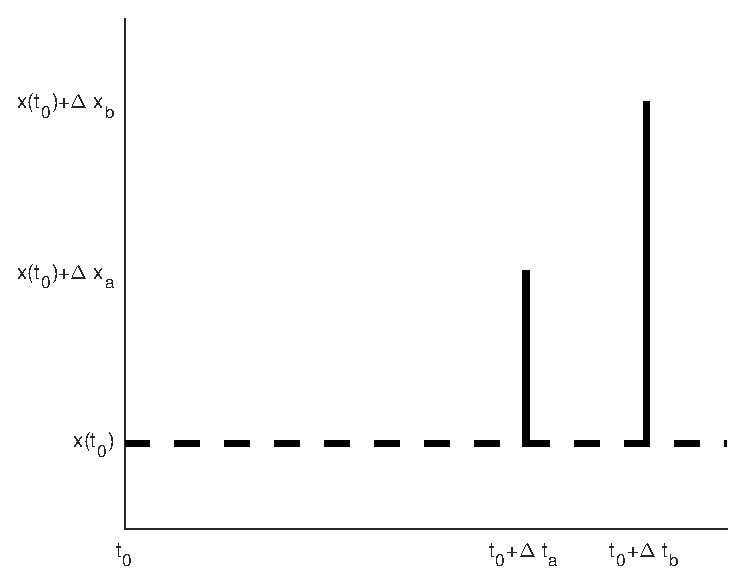
\includegraphics[width=0.75\textwidth]{./figures/basicsetup.eps}
\caption{The basic setup of the model. A decision maker faces a choice at time $t_0$ between option $a$, which guarantees a payoff of $\Dx_a$ after time period $\Dt_a$, and option $b$, which guarantees a payoff of $\Dx_b$ after time period $\Dt_b$.}
\flabel{basicsetup}
\end{figure}

We note that in this setup there is no uncertainty in the payoffs or in the times in which they are realized. Thus, there is no risk.
%Because there is no risk, we do not specify a utility function and consider the dollar value of the payoffs.

This setup corresponds to a standard question that arises in the context of temporal discounting, \eg ``would you prefer to receive \$100 tomorrow or \$200 in a month's time?'' Despite its apparent simplicity, answering this question requires additional assumptions. One such assumption concerns the dynamics under which the decision maker's wealth grows. A common assumption is that it grows exponentially, compounding continuously at a risk-free rate like funds in a savings account. Another assumption is the time frame of the decision, specifically whether a decision to accept the earlier payout is treated as playing out over $\Dt_a$ only, or over the full period $\Dt_b$. XXXOP or over some other $\Delta t$? As $\Delta t \to \infty$ all growth rates go to zero, and our framework becomes degenerate (it can't select an optimum). This could be interpreted as the one-shot setup.XXX
Such assumptions are needed to permit computation of the decision maker's maximand -- in our model, the growth rate of his wealth -- so that the options can be compared quantitatively.

We will describe four different specifications of this basic setup. In each we will calculate the growth rates, $g_a$ and $g_b$, of total wealth associated with options $a$ and $b$. The decision maker compares the two growth rates and prefers the option whose growth rate is larger.

From this comparison can be also inferred the discount factor (\textit{DF}). This is the multiplicative factor, $\delta$, by which the later payout, $\Dx_b$, must be multiplied to equal the earlier payout, $\Dx_a$, when the payout amounts and times are such that the decision maker is indifferent between the two options. In symbols,

\be
\delta \equiv \frac{\Dx_a}{\Dx_b}
\ee
under indifference.
%To calculate to DF, we evaluate the ratio between the payout $\Dx_a$ and the payout $\Dx_b$ under the assumption that the the growth rates $g_a$ and $g_b$ are equal.

As we show below, this setup predicts decisions equivalent to hyperbolic and exponential discounting under different specifications. Some specifications of the model predict preference reversal. Our model differs from many standard models in the literature by assuming that decision makers maximize the growth rate of their wealth, rather than the expected change in their utility.
%It has been shown to be equivalent in some cases, under specific dynamics and specific utility function choices~\citep{peters2018time}. It is further discussed in~\Sref{discussion}.

\section{Results}\label{sec:results}

We begin by describing four different specifications for our basic setup. Each specifies two aspects necessary to quantify the growth rate of wealth: the time frame of the decision; and the dynamics under which wealth evolves.

The time frame is a key aspect, often left unspecified in similar setups in the literature. Consider the following scenarios:

\begin{enumerate}
    \item Dana, the real estate developer, loves to work and always wants to keep busy with her building projects, she always gets paid at their completion. Dana has a choice between a project that lasts three months and a project that lasts six months. 
    \item Every year, Nate the Naval officer must go for either a three month long mission or a six month long mission. He is given the choice at the beginning of every year(both missions finish before the end of the year). He is paid right after his mission is completed.
\end{enumerate}

In the first scenario, the time frame depends on the choice made. We call this the \textit{elastic} time frame because Dana is more flexible to pursue other opportunities if she chooses the shorter project. On the other hand, if she chooses the longer project, it locks her in a for a longer time period, which means it also changes when she will have another choice.  

In the second scenario, the important element to note is that no matter which choice is made, it will not affect future choices, said otherwise, the time frame is independent of the choice, it is \textit{fixed}. That is, the timing of Nates next choice is not affected by his decision. 

In our model, we must choose the time frame over which the growth rates of wealth in each option are computed. We can choose it to be the time period associated with each payout, \ie $\Dt_a$ for option $a$ and $\Dt_b$ for option $b$. This specification corresponds to Dana's choice, the elastic time frame specification. Or we can choose it always to be the longer time period, $\Dt_b$, resembling Nate's dilemma, the fixed time specification. 

%\textcolor{red}{\begin{enumerate}
%    \item A builder must choose between two jobs starting tomorrow, one paying \$1,000 for a week's work and the other paying \$3,000 for a month's work, with both sums being paid on completion of the work.
%    \item An author must choose %between receiving \$30,000 in advance or \$50,000 on production of a book that will take a year to write.
%\end{enumerate}}


% \textcolor{red}{In the first scenario, the time frame depends on the choice made: one week for the smaller job; one month for the larger job. If the builder chooses the smaller job, he is free to pursue other opportunities during the three-and-a-bit weeks between its completion and the completion of the larger job. But if he chooses the larger job, he can do nothing else for the whole month. Although the guaranteed payout is greater, the larger job has an opportunity cost relative to the smaller one.}

%\textcolor{red}{In the second scenario, the time frame is independent of the choice: in both cases, the author must work for one year. In particular, taking the earlier payout does not allow her (ethically, at least) to pursue other opportunities during the period between it and the later payout that she declined.}


%\textcolor{red}{In our model, we must choose the time frame over which the growth rates of wealth in each option are computed. We can choose it to be the time period associated with each payout, \ie $\Dt_a$ for option $a$ and $\Dt_b$ for option $b$. This specification reminds us of the builder's choice and we will call it the elastic time frame specification. Or we can choose it always to be the longer time period, $\Dt_b$, resembling the author's dilemma. We will call this the fixed time frame specification.}

%One possibility is to assume a fixed time frame -- the decision maker faces the choice every $\Dt_b$. In this case, in order to compare between the two choices, we will evaluate the growth rates between $t_0$ and $\Dt_b$ in both options. Another possible specification of time frame, is that the decision maker faces a choice after the payoff is exercised, \ie after $\Dt_a$ if option $a$ was chosen and after $\Dt_b$ if option $b$ was chosen. In this case, we will evaluate the growth rate for option $a$ at time $\Dt_a$, and for option $b$ at $\Dt_b$. The former time frame will be labeled the fixed time frame and the latter the elastic time frame.

The wealth dynamics can also take different forms. A standard assumption would be that wealth grows exponentially in time, assuming a risk-free rate $r$. We label this dynamic as multiplicative. This dynamic corresponds to investing wealth in income-generating assets, in which the income is proportional to the amount invested. This is the dynamic traditionally assumed in temporal discounting, and when present values are calculated for future expected payouts. In this case it is also assumed that the payout itself is re-invested at the risk-free rate.

Another possible form is additive dynamics. Under this dynamic wealth grows linearly in time, with a rate $k$, and it is not invested in income-generating assets. It is equivalent to assuming a flow of wealth at some rate, \ie labor income. In this case, there is essentially no re-investment of the payout -- the income generated by this dynamic is not proportional to wealth as in the multiplicative dynamics.
%As we will see, this is equivalent to assuming no wealth dynamics, \ie that wealth does not grow in time, apart from the changes that are due to the payouts.

The definition of the wealth growth rate differs for the different dynamics. The growth rate between time $t$ and $t+\Dt$ under additive dynamics is $\frac{x\left(t+\Dt\right)-x\left(t\right)}{\Dt}$ and under multiplicative dynamics it is $\frac{\log x(t+\Dt)-\log x(t)}{\Dt}$, see also~\citep{peters2016evaluating,peters2018time}.

We will discuss the four specifications, as illustrated in~\fref{tree}. In each case we will: compute the growth rates $g_a$ and $g_b$ associated with each option; compare them to determine the conditions under which each option is preferred; elicit the form of temporal discounting equivalent to our decision model; and, finally, determine whether PR is predicted.

\begin{figure}[!htb]
\centering
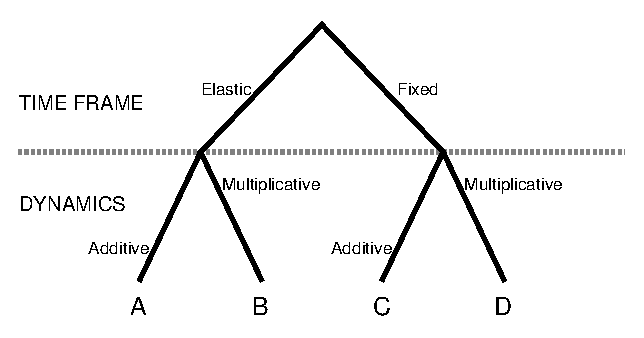
\includegraphics[width=0.75\textwidth]{./figures/tree.eps}
\caption{The four model specifications, determined by specifying a time frame and wealth dynamics. The labels A, B, C, and D, are used for the different cases.}
\flabel{tree}
\end{figure}

\subsection{Case A -- Elastic time frame with additive dynamics}\label{sec:case_A}

Specification: the time frame for computing the growth rate is time to the chosen payout; and the wealth dynamics are additive (with growth rate $k$). We begin by writing down the final wealth under the two options, evaluated at $t_0+\Dt_a$ and $t_0+\Dt_b$ respectively:
\bea
x\left(t_0+\Dt_a\right) &= x\left(t_0\right) + \Dx_a + k \Dt_a\,;\\
x\left(t_0+\Dt_b\right) &= x\left(t_0\right) + \Dx_b + k \Dt_b\,.
\eea

The growth rates are:
\bea
g_a &=& \frac{x\left(t_0+\Dt_a\right) - x\left(t_0\right)}{\Dt_a} = \frac{\Dx_a}{\Dt_a} + k\,;\\
g_b &=& \frac{x\left(t_0+\Dt_b\right) - x\left(t_0\right)}{\Dt_b} = \frac{\Dx_b}{\Dt_b} + k\,.
\eea

It follows that the criterion $g_a > g_b$ is
\be
\frac{\Dx_a}{\Dt_a} > \frac{\Dx_b}{\Dt_b}\,.
\ee

This criterion suggests that under this specification, the only thing that matters to the decision maker is the payout rate of each option with respect to the reference point in time, $t_0$. The same payouts would translate into different payout rates for each option with a different reference point in time. This, in turn, would allow for preference reversal. This is illustrated in~\fref{caseA}.

\begin{figure}[!htb]
\centering
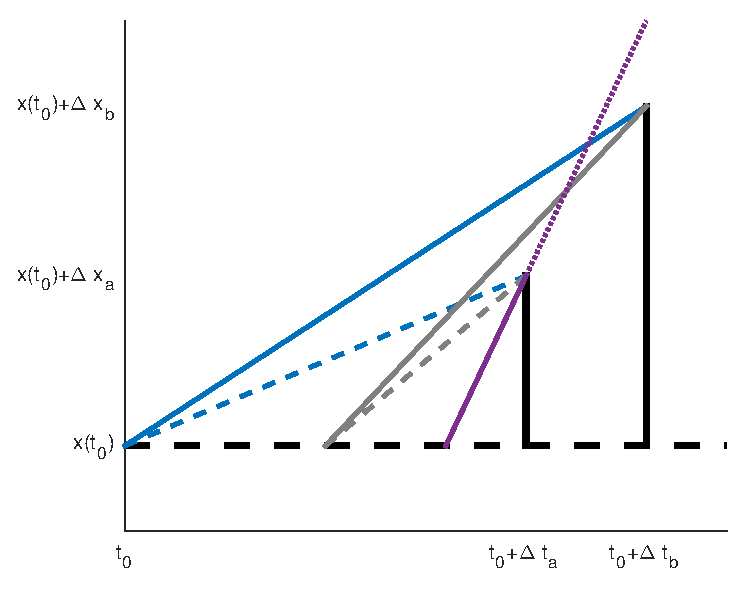
\includegraphics[width=0.75\textwidth]{./figures/case_A.eps}
\caption{An illustration of preference reversal in case A. Initially, option $b$ is preferable. It is reflected in the slopes of the blue lines. The solid blue line shows the payout rate of option $b$ and the dashed blue line shows the payout rate of option $a$. Even after some time, option $b$ is still preferable, as reflected by the difference in the slopes of the gray lines (solid for option $b$, dashed for $a$). At some point option $a$ becomes preferable, as the payout rate surpasses that of option $b$. This is demonstrated in the purple line.
XXXOP something is not right with this figure. I like the different colors for different times. Perhaps let's have one case preferences 1, one case equanimity, one case preferences 2.XXX}
\flabel{caseA}
\end{figure}

It shows that the payout rate of option $b$ is higher than that of option $a$, which makes it preferable. This holds for some time. However, at some point in time, this changes and the payout rate of option $a$ would be higher. Assuming that initially option $g_b > g_a$, there will always be a point in time in which PR will occur. If time $\tau$ elapsed from $t_0$, than the updated payout rates of options $a$ and $b$ are $\frac{\Dx_a}{\Dt_a - \tau}$ and $\frac{\Dx_b}{\Dt_b - \tau}$, respectively. The reversal will occur when these are equal, or
\be
\tau_{\text{reversal}} = \frac{\Dt_a\Dx_b - \Dt_b\Dx_a}{\Dx_b - \Dx_a}\,.
\ee

This case not only demonstrates PR, but also hyperbolic discounting, \ie that the discount factor changes hyperbolically in time.

The discount factor, $\delta$, is the factor by which the later payout, $\Dx_b$, must be multiplied to equal the earlier payout, $\Dx_a$, under indifference between options $a$ and $b$. Practically, it can be found by considering the equality of growth rates $g_a$ and $g_b$, which is the condition for indifference. $\delta$ is typically presented as a function of the time difference between options. In our setup this would be $\Epsilon \equiv \Dt_b - \Dt_a$.

\textcolor{red}{
Now that we have the hyperbolic DF in terms of the delay, $\Dt_b-\Dt_a$, and the time to the first payout, $\Dt_a$, as
\be
\delta = \frac{1}{1+\frac{\Dt_b-\Dt_a}{\Dt_a}} = \frac{1}{1+kD},
\ee
it would be much clearer to present PR as a consequence of changing the time to the first payout rather than the reference time. Then $t_0\to t_0+\Dt_a$ is simply $\Dt_a\to0$, which is also expressible as $k\to\infty$. This minor reframing will require some changes below, including to the figure, because we would treat $t_0$ as fixed and $\Dt_a$ as movable.
}
\textcolor{red}{
Do we need $\Epsilon$? The letter has no intuitive meaning (to me) and perhaps we can get away without relabelling $\Dt_b-\Dt_a$. If not, $D$ for delay or $W$ for wait might be better.
}
XXXOP: not sure -- I like the physical time $t_0$ changing. What happens in real life is that time ticks on and we get swept towards $t_a$, it's not that we sit still in time, and someone tunes $t_a$. Agree about $\Epsilon$ -- better letter?XXX


In case A we therefore get
\be
\delta_A = \frac{\Dx_a}{\Dx_b} = \frac{\Dt_a}{\Dt_b} = \frac{1}{1+\frac{1}{\Dt_a} \Epsilon}\,.
\ee

This is exactly hyperbolic discounting with degree of discounting $\kappa = \frac{1}{\Dt_a}$.

We note also that, under additive dynamics, the background growth rate, $k$, of the decision maker's wealth does not appear in the decision criterion. This is because wealth growth under additive dynamics is not affected by exogenous cash flows: the gain $k\Dt$ over period $\Dt$ occurs regardless of what else happens. This contrasts with multiplicative dynamics, where early cash flows can be reinvested to increase gains from growth.

\subsection{Case B -- Elastic time frame with multiplicative dynamics}\label{sec:case_B}

Specification: the time frame for computing the growth rate is time to the chosen payout; and the wealth dynamics are multiplicative (with growth rate $r$). We follow the same steps as in case A. Wealth evolves to:
\bea
x\left(t_0+\Dt_a\right) &= x\left(t_0\right) e^{r \Dt_a} + \Dx_a\\
x\left(t_0+\Dt_b\right) &= x\left(t_0\right) e^{r \Dt_b} + \Dx_b\,.
\eea

The corresponding growth rates are:
\bea
g_a &= \frac{1}{\Dt_a} \log{\left(\frac{x\left(t_0+\Dt_a\right)}{x\left(t_0\right)}\right)} = \frac{1}{\Dt_a}\log{\left(e^{r \Dt_a} + \frac{\Dx_a}{x\left(t_0\right)}\right)}\\
g_b &= \frac{1}{\Dt_b} \log{\left(\frac{x\left(t_0+\Dt_b\right)}{x\left(t_0\right)}\right)} = \frac{1}{\Dt_b}\log{\left(e^{r \Dt_b} + \frac{\Dx_b}{x\left(t_0\right)}\right)}\,.
\eea

This setting also displays PR, although no closed-form expression for $\tau_{\text{reversal}}$ can be derived like in case A. It is clear that PR occurs, since when $\tau$ approaches $t_0+\Dt_a$, $g_a$ will increase indefinitely, while $\log{\left(e^{r \Dt_a} + \frac{\Dx_a}{x\left(t_0\right)}\right)}$ remains positive.

Similarly, the discount factor $\delta_B$ cannot be derived explicitly without approximations. Yet, we could assume that $\Dx_a \ll x\left(t_0\right)e^{r \Dt_a}$ and $\Dx_b \ll x\left(t_0\right)e^{r \Dt_b}$, \ie that the payouts are much smaller than the wealth at the time the payouts are realized. Then, using the first order expansion $\log\left(x+\delta\right) \approx \log\left(x\right) + \delta/x$, we obtain

\be
\delta_B = \frac{\Dx_a}{\Dx_b} \approx \frac{\Dt_a}{\Dt_b} \cdot e^{-r \left(\Dt_b - \Dt_a\right)} = \frac{1}{1+\frac{1}{\Dt_a} \Epsilon}e^{-r\Epsilon}\,,
\ee

which is a mixed case of hyperbolic and exponential discounting.

\subsection{Case C -- Fixed time frame with additive dynamics}\label{sec:case_C}

Now we assume additive dynamics again, but with a fixed time frame -- the outcomes of both choices are compared at $\Dt_b$. The growth rate of option $b$ would be the same as in case A, since it was already evaluated at $t_0+\Dt_b$. In this case, option $a$ leads to
\be
x\left(t_0+\Dt_b\right) = x\left(t_0\right) + \Dx_a + k \Dt_b\,,
\ee

and the corresponding growth rate would be
\be
g_a = \frac{1}{\Dt_b}\left(x\left(t_0+\Dt_b\right) - x\left(t_0\right)\right) = \frac{\Dx_a}{\Dt_b} + k\,.
\ee

Recall that $g_b = \frac{\Dx_b}{\Dt_b} + k$. Since we have assumed $\Dx_b > \Dx_a$, it is clear that option $b$ would always be preferable to option $a$. This is a trivial case -- assuming additive dynamics (or no dynamics) the only thing that matters is the payout size, if we compare the options at the same time, or if they repeat at fixed time windows. In this case, the discount factor $\delta_C$ cannot be defined, since the larger final payout is always preferred and the indifference condition cannot be satisfied.

\subsection{Case D -- Fixed time frame with multiplicative dynamics}\label{sec:case_D}

Finally, we assume multiplicative dynamics and a fixed time frame. This is the specification that corresponds to the standard assumptions usually considered in temporal discounting -- that wealth is continuously compounding at the risk-free rate and that payouts are re-invested at this rate.

The growth rate of option $b$ would be the same as in case B, since it was already evaluated at $t_0+\Dt_b$ ($g_b = \frac{1}{\Dt_b}\log{\left(e^{r \Dt_b} + \frac{\Dx_b}{x\left(t_0\right)}\right)}$). In this case, option $a$ leads to
\be
x\left(t_0+\Dt_b\right) = x\left(t_0\right) e^{r \Dt_b} + \Dx_a e^{r \left(\Dt_b - \Dt_a\right)}\,,
\ee

and the corresponding growth rate would be (recall that $\Epsilon \equiv \Dt_b - \Dt_a$)
\be
g_a = \frac{1}{\Dt_b} \log{\left(\frac{x\left(t_0+\Dt_b\right)}{x\left(t_0\right)}\right)} = \frac{1}{\Dt_b}\log{\left(e^{r \Dt_b} + \frac{\Dx_a e^{r \Epsilon}}{x\left(t_0\right)}\right)}\,.
\ee

It follows that the criterion $g_a > g_b$ is
\be
\Dx_a e^{r \Epsilon} > \Dx_b\,.
\ee

The discount factor can be then easily calculated by considering the equality of the growth rates. In this case we get $\Dx_a e^{r \Epsilon} = \Dx_b$ and therefore
\be
\delta_D = \frac{\Dx_a}{\Dx_b} = e^{-r\Epsilon}\,,
\ee
which is the standard exponential discounting result. In other words, if it is possible to re-invest the reward given at time $\Dt_a$ so that it surpasses the alternative reward given at time $\Dt_b$, option $a$ is preferable over option $b$, and vice versa.

\section{Discussion}\label{sec:discussion}

This paper describes a model in which a decision maker chooses between two payoffs realized at different points in time by comparing the growth rate of wealth associated with each option.

The main finding is that discounting can be interpreted as growth rate optimization. We find that depending on the wealth dynamics assumed by the decision maker, growth rate optimization can be equivalent to hyperbolic discounting, in which case it predicts preference reversal. It can also be equivalent to a mixed case of hyperbolic and exponential discounting, which also implies preference reversal. Under multiplicative dynamics, we find that growth-rate optimization reproduces standard exponential discounting. This reveals the standard form of discounting as just one of many possible forms of discounting, each of which is optimal under a different type of wealth growth.

A fundamental question about the model is why would someone maximize growth instead of expectation value of utility? This, of course, differs from the traditional framework for analyzing decisions in economics, usually taking it as axiomatic that people maximize utility. Yet, this is only one way of studying optimal choice under different conditions. At the same time it is important to question where does the utility optimizing mechanism come from?

The framework we used here has an answer -- evolutionary mechanisms. That is, some utility functions survive better than others. The utility functions that will survive over the long run are the growth utility functions.

This paper discusses discounting from a theoretical perspective. An important complementary step of this research would be comparing the theoretical predictions of the results to empirical and experimental results. In particular, the predicted discount factors and discount rates can be compared to results from controlled experiments. This is planned for future work.

An additional extension is the inclusion of risk. The standard explanations to hyperbolic discounting consist of a behavioral response to risk~\citep{sozou1998hyperbolic,dasgupta2005uncertainty}, while here we showed that hyperbolic discounting can be observed even in the absence of uncertainties in the payouts or in their timing. Adding uncertainty to our model might create additional forms of temporal discounting, which might be more realistic and closer to empirical evidence.

\textcolor{green}{Given the framework here, risk can be interpreted in two ways. Either it represents the actual probability of an arrival of a choice or it represents the belief about the environment. The corresponding discount rate then be some weighted average between the discount rates presented here. }

%Though utility functions are traditionally used for individuals, this framework implies that even firms should have utility functions. That is, why should firms discount hyperbolically? If a firm has a fixed staff and cannot undertake numerous projects at the same time and has access to some interest rate, then it should discount hyperbolically. If the evolutionary mechanism is considered, maximizing the expected value can actually be considered as merely a case of bounded rationality. The process of updating beliefs based solely on observation without reference to the environment, may be ecologically irrational.

%Whether actual decision makers behave this way is an empirical question, nevertheless this theory relative to the classic case, has more Popperian content inscribed in it. So we consider that this framework offers a rich agenda for research. Yet, the empirical implications of the model do have falsifiable content. That is, after we observe a specific discount factor from someone, we can deduce the environment they are in. For instance, if someone is in a changing environment, we should expect them use the ensemble average. If, on the other hand, the environment is constant then we predict that they will behave more like the time average. An objective measure of opportunity could be one way to construct such a measure.

%This is only one way to interpret the model. Another way would be that the preferences which are revealed, also reveal a belief set. However, this case is not as empirically interesting because the belief set is defined by the preferences and does not imply a cognitive awareness of the implied belief. That is, just because a set of beliefs are implied, this does not mean that they can be solicited. Why might we not be able to solicit preferences? For it to be possible to solicit preferences it must assumed that the decision rule used in experiments is the same as the one used in the real world. Well how do we verify that the actual preferences are the same ones as the ones that were solicited? By looking to see consistency between solicitation and the real world. 

%It is possible to find that agents make use of a specific decision rule only for such experiments. We then should ask why do some people change their decision rules when solicited whilst others do not? Ultimately, this question must be answered without looking at solicited preferences. So there is still a need to look at the environment of the agent. Focusing on beliefs does not in fact ever yield satisfactory answers because the meta question will always exist.

%Using solicited preferences does in fact requires going back to the real world in any case, so it can be skipped altogether. The approach in this paper differs by offering the potential to omit the solicitation. Observing data on how decision makers make investment choices in the real world, can describe the discount rate. If we cannot tell which specification of the model should be used, more information may be used. For instance, if someone has access to a good investment manager or if they often have investment opportunities. The advantage of this approach is to bypass the need to look at verbally stated beliefs.

\newpage

\bibliography{discountingbib}

%\clearpage
%
%\appendix
%
%\section{???????????}
%\label{app:appA}

\end{document}